% Publication: EIDORS: uses and abuses
% Authors: Andy Adler, Bill Lionheart
% $Id: adler-lionheart-2005-EIDORS.tex,v 1.22 2005-11-03 16:50:31 aadler Exp $
\documentclass[12pt]{iopart}
%Query macro
\newcommand{\query}[1]{%
    \marginpar{%
      \hrule height1pt
      \vspace*{4pt}
      {\raggedright\scriptsize\slshape #1\par}%
      \vspace*{4pt}
      \hrule height1pt
    }%
}

\usepackage[dvips]{graphicx} % Package for inserting figures
\begin{document}
\title{Uses and abuses of EIDORS: An extensible software base for EIT}
\author{Andy Adler$^1$, William R. B. Lionheart$^2$}
\address{$^1$ School of Information Technology and Engineering (SITE), University of Ottawa, Canada}
\address{$^2$ School of Mathematics, University of Manchester, U.K.}
\eads{
   \mailto{adler@site.uOttawa.ca}
   \mailto{bill.lionheart@manchester.ac.uk}
     }

\begin{abstract} %Single paragraph text only (no ref. eqn. max.200 words)

EIDORS is an open source software suite for image reconstruction in
electrical impedance tomography and diffuse optical tomography;
designed to facilitate collaboration, testing and new research
in these fields.  This paper describes recent work to
redesign the software structure in order to simplify its use
and provide a uniform interface,
permitting easier modification and customization.
We describe the key features of this software, followed by
examples of its use.
One general issue with inverse problem software is the difficulty
of correctly implemeting algorithms, and the consequent ease with
which subtle numerical bugs can be inadvertently introducted.
EIDORS helps with this issue, by allowing sharing and reuse
of well documented and debugged software. On the other hand, 
EIDORS potentially encourages such issues by facilitating use
by non-specialists. In order to address this issue, we develop
a list ``cheats'' with inverse problems. Our hope is that such
a list will assist authors of software to avoid such implemention
issues.


\end{abstract}
\noindent{\it Keywords\/}:
Electrical Impedance Tomography,
Open Source,
Inverse Problems

\section{Introduction}

EIDORS
({\bf E}lectrical
 {\bf I}mpedance and
 {\bf D}iffuse
 {\bf O}ptical tomography
 {\bf R}econstruction
 {\bf S}oftware )
is a software suite for image reconstruction in
electrical impedance tomography and diffuse optical tomography.
The goal is to provide a freely distributable and modifiable
software for image reconstruction of electrical 
or diffuse optical data. Such software facilitates research
and development
in these fields by providing a reference implementation
against which new developments can be compared, and by
providing a functioning software base onto which new
ideas may be built and tested.
Making the source code available also facilitates scrutiny
of algorithms and their implementation by other researchers.
The original EIDORS (version 1) software (\cite{Vauhkonen_etal_2000})
is based on software from the thesis of Vaukhonen \cite{Vauhkonen_1997}
It implemented a MATLAB package for two-dimensional mesh generation,
solving of the forward
problem and reconstruction and display of the images.
In order to provide capability to solve 3D reconstruction models,
a new project, EIDORS3D (version 2), was begun \cite{Polydorides_and_Lionheart_2002},
based on the software developed for thesis of Polydorides \cite{Polydorides_2002}
The EIDORS software packages shared the same numerical
and algorithmic foundations, but shared very little software code.
Each software package modelled the medium under investigation
using a simplex based finite element representation,
and images were reconstructed using regularized inverse techniques.

In the three years since the publication of EIDORS3D, several patterns
of use have been noted. Researchers typically download the software,
run the provided demonstration examples,  and 
make modifications in the demonstration examples and the software
internals to meet their needs.
Because of the lack of a modular software structure of EIDORS3D,
changes tended to made into the code itself. This resulted in
duplicated
code which could not easily be {\em refactored} in order to
be contributed back to EIDORS. Additionally, recent work has begun to move
away from basic reconstruction algorithms, focussing
on such issues as mesh generation, electrode modelling, visualization
and electrode error detection. This research would be facilitated
by using modular components which could be {\em plugged} into
a selection of reconstruction algorithms.

To address these issues, the EIDORS software has been completely
restructured with the goal of providing an {\em extensible software base}
designed to support {\em community} use, modification and contribution.
These modifications have been released as EIDORS version 3.0,
which incorporates the following features:

\begin{itemize}

  \item {\em Multiple algorithm support:}
EIDORS V.3 has been redesigned to allow flexibility of
using multiple algorithms (or parts of algorithms). 
This version provides access to the algorithms of
\cite{Adler_and_Guardo_1996}, \cite{Polydorides_and_Lionheart_2002},
\cite{Soleimani_etal_2005} and \cite{Vauhkonen_etal_2000}.
We feel that this capability is becoming more
important with a trend toward meta-algorithms
in EIT, such as algorithms for detection of
electrode errors \cite{Asfaw_and_Adler_2005}. 

  \item {\em Generalized data formats:}
One limitation of previous versions of the EIDORS software
is that they were designed around specific electrode configurations
and stimulation and measurements patterns. While it was possible
to use the software for more general configurations, this was 
a fairly daunting task. In order to support the wide
variety of EIT measurements and algorithms, EIDORS now provides
a general EIT data format (the {\tt fwd\_model} structure).
Additionally, several utility functions are provided to
create common electrode and stimulation configurations.
This format specifies the electrode positions, contact impedances,
and stimulation and measurement patterns, and all supported
algorithms are able to reconstruct images based on data
provided in these formats.

  \item {\em Interface software for common EIT systems:}
functions are provided (in the {\em interface} directory) to load
from a variety of EIT hardware storage formats into the
EIT data format. Currently, EIDORS will detect when data
does not match the specified protocol in the {\tt fwd\_model},
but will not (yet) automatically convert the data.
At this point it has only been possible for the developers to 
offer support for EIT hardware that they have access
to. We hope that EIDORS will attract contributions from
software developers who have access to other hardware
systems.

  \item {\em Usage examples:}
It is observed that researchers typically base new software on
demonstration examples. To facilitate this, some simple and more
complex usage examples are provided for image reconstruction
in two-and three dimentions using various image reconstruction
algorithms and combinations of algorithms.

  \item {\em Test suite:}
Software is intrinsically difficult to test. While little work
has been done specifically on testing numerical software
for inverse problems, we
believe that such tests are even more difficult.
EIDORS has begun to implement a series of regression test
scripts (in the {\tt tests} directory)
to allow automatic testing of code modifications.
For example the function {\tt calc\_jacobian\_test.m}
validates a function to calculate the Jacobian against
a calculation using the perturbation method. 

  \item {\em Open-source license:}
EIDORS is licensed under the
GNU General Public License \cite{Free_Software_Foundation_1991}.
Users are free to use, modify, and
distribute their modifications. All modifications must include the
source code, or instructions on how to obtain it. EIDORS may be used
in a commercial product, as long as the source code for EIDORS and all
modifications to it are made available.

  \item {\em Sourceforge hosting:}
In order to allow collaborative development, 
EIDORS is hosted by {\tt sourceforge.net}
available at {\tt http://eidors3d.sf.net}.
Software is available for download as packaged released versions
(version 3.0 was released on 31 Oct 2005, and
contains the features described in this paper),
or the latest developments may be downloaded from the
Concurrent Versions System (CVS) \cite{Cederqvist_2002}.
Sourceforge hosting allows for collaborative development for
group members, while permitting read-only access to everyone.
In order to become a member of the developer group, new
contributors should contact the authors.
One concern with a distributed software project is
the possibility of conflict due to disparate authors
working on the same module.
Version control software such as CVS is widely understood
to facilitate collaborative development, and manage
software version conflicts.


  \item {\em Language independence: (Octave and Matlab)}
EIDORS was originally written for Matlab.
However, the eventual goal is to support multiple
mathematical software packages.
Some progress has been achieved, and EIDORS version 3
works with Octave \cite{Eaton_2002}, although some 
advanced graphics functions still function only with Matlab.
The current version of EIDORS works with Octave
(version $\ge$ 2.9.3)
and Matlab (version $\ge$ 6.0).
Support for octave was motivated by two goals:
first, octave provides a free software platform
which can encourage the development of embedded
and commercial applications of EIT
are limited by the cost of Matlab, and secondly
octave provides an open source platform to match
the open source nature of EIDORS.

  \item {\em Pluggable code base:}
In order to facilitate user modifications, EIDORS
has been designed to provide some of the benefits of
object-oriented (OO) software \cite{Gamma_etal_1995}:
{\em abstraction}, {\em encaptulation}, 
{\em polymophism} and {\em inheritance}.
We have decided not to
use the OO framework provided by Matlab, because
in our experience it is somewhat cumbersome,
and may be intimidating
to many mathematicians and engineers who do not 
regularly write OO software.
Another issue is the unfortunate reputation of
Matlab for making dramatic modifications to new
language features in the first few versions.
For these reason, EIDORS has been designed using
a  ``Pluggable'' software approach.
This design uses function
pointers to allow adding new modules and controlling
which parts of functions are executed.
EIDORS is thus able to offer the OO features 
of {\em packaging}, and {\em polymophism}, while
not {\em encaptulation} or {\em inheritance}.
A detailed description of this capability is
provided in the next section.

  \item {\em Automatic matrix caching:}
In order to increase
performance of image reconstruction software, it is important to save
and reuse values of 
computationally expensive variables, such as the Jacobian and image priors.
Such caching complicates the software implementation, and
potentially leads to errors. In order to simplify design, EIDORS
offers the ability to automatically detect when a calculation
requests a value previously calculated, and will automatically
retrieve that previous value.
EIDORS extracts caching to a separate module {\tt eidors\_obj},
in a way that will generally happen transparently for the
programmer. This capability helps software based on EIDORS
to be cleaner and easier to decompose into functional
modules.


  \item {\em Enhanced Finite Element Modelling and Graphical output:}
Image reconstruction, especially in 3D, requires functions
to show high quality graphical representations of the images.
EIDORS provides several functions for image presentation:
{\tt show\_fem.m} displays a three dimentional model of the
finite element mesh and conductivity changes, while
{\tt show\_slices.m} allows generation of images of arbitrary
two dimentional slices through a volume. Examples of these
functions are shown in \ref{fig:fig_3d_zigzag} and \ref{fig:fig_3d_2rings}.
All EIDORS graphics functions now use a single colour
mapping function {\tt calc\_colours.m}, which allows
global modification of all image colouring using a
global variable {\tt eidors\_colours}.


%  \item {\em Logo:}
%Since EIDORS images blobby objects in aqueous media,
%the logo \label{fig:logo}, was chosen to be a walrus,
%since it is (also)
%a fat, blobby animal that lives in water.
%
%%
%% FIGURE: EIDORS LOGO
%%
%\begin{figure}[th]
%\begin{flushright}
%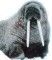
\includegraphics[width= 0.40 \textwidth]{./figs/eidors-logo.eps}
%\caption{\small EIDORS logo.
%{\em EIT}: images blobby objects in aqueous media;
%{\em Walrus}: a fat, blobby animal that lives in water.
% Images credit: (C) Genny Anderson {\tt www.biosbcc.net} 
% }
%\end{flushright}
%\end{figure}

\end{itemize}
We hope that by providing a structure for community collaboration
in EIT algorithms, we can produce robust,
reliable and fairly portable software which draws on our collective
expertise and facilitates innovations in the field.

\section{Software Architecture}

\subsection{Object Structure}

EIDORS software consists of four primary objects:
{\tt data},
{\tt image},
{\tt fwd\_model},
{\tt inv\_model}. Each object is represented by a
structure. All objects have the properties of a
{\tt name} and {\tt type}. The {\tt name} is
arbirary; it is displayed by the graphics functions,
used could also be be useful to distinguish objects
in a user specified function. The {\tt type} must
be one of the primary objects. In this section we
consider each software object and its properties.


All EIDORS objects are represented using as a Matlab
(or Octave) structure. All objects must have 
{\tt name} and {\tt type} fields. 
The {\tt type} is used to identify the object type 
(ie {\tt data}, {\tt image} etc.).
The {\tt name} is arbirary, and may be used or ignored
by software using EIDORS; it is only used by the
graphical functions of EIDORS to anotate displayed images.

\subsubsection{fwd\_model}

%
% FIGURE: Forward Model
%
\begin{figure}[th]
\begin{flushright}
\includegraphics[width= 0.50 \textwidth]{./figs/fig_model2.eps}
\caption{\small The structure of the EIDORS {\tt fwd\_model} object.
\label{fig:fwd_model}
 }
\end{flushright}
\end{figure}


The most complex EIDORS object is the {\tt fwd\_model},
which is designed to represent the finite element model 
(FEM), electrode
positions and properties, and stimulation patterns, as
well as the pointers to functions to solve the forward
problem on this model. Fig. \ref{fig:fwd_model} illustrates
the structure of a {\tt fwd\_model}.

The FEM is described by the fields
{\tt nodes} ($V{\times}D$),
{\tt elems} ($N{\times}(D+1)$), and
{\tt boundary} ($B{\times}D$), where
$V$ is the number of vertices, $N$ is the number of
simplices (and also the number of unknown conductivities
to be solved by the inverse solution), $B$ the number
of simplices with a face on the boundary, and $D$ the
model dimention ($D=2$ for 2D and $D=3$ for 3D).
The {\tt gnd\_node} is the vertex number attached to ground.

The electrodes are defined by a vector ($E\times1$) of
{\tt electrode} fields. Each of $E$ {\tt electrode}
objects has fields
{\tt z\_contact} (scalar) and {\tt nodes} (vector)
 which represent the
(possibly complex) contact impedance
and vertices to which that electrode is connected.
A point electrode would have a single element
{\tt nodes} field with ${\tt z\_contact}=0$ while
an electrode with a complete electrode model
would have multiple vertices specified in {\tt nodes}
and ${\tt z\_contact}\ge0$. Note that EIDORS
does not require the electrode model to be the same
for all electrodes in a {\tt fwd\_model}.

Using these electrodes, a sequence of $S$ stimulation
patterns are applied and measurements are performed
in order to generate a frame of data.
Stimulation patterns are defined by a vector
($S\times1$) of {\tt stimulation} fields. Each
{\tt stimulation} object has fields
{\tt stimulation}, 
{\tt stim\_pattern}, and
{\tt meas\_pattern}. The {\tt stimulation} is
the quantity stimulated into the electrodes. Typically,
EIT systems inject current (represented by ``mA''),
but the quantity could be voltage (or luminous
intensity in an optical tomography system). Currently,
EIDORS only accepts current stimulations.
{\tt stim\_pattern} is a vector ($E\times1$)
of the stimulation quantity applied to each electrode
during that stimulation pattern.
{\tt meas\_pattern} is a (sparse) matrix ($E{\times}M_i$) 
representing the $M_i$ measurement patterns for
stimulation $i$. Each column of this matrix represents
the amplification of the signal at each electrode for
a single measurement pattern. For example if measurement
$k=2$ is the difference signal between electrodes 4 and 5,
then ${\tt meas\_pattern}_{j,k}$ is $1$ for $j=4$,  $-1$
for $j=5$ and zero for other values of $j$ when $k=2$.
EIDORS does not require that the number of measurement
patterns be equal for each stimulation pattern. 
The total number of measurements per frame is
$ M = \Sigma_{i=0}^{S} M_i$

For many EIT systems, an adjacent stimulation
pattern is used with no measurement taken at current
stimulation electrodes, giving $M = E\times(E-3)$.
For a $16$ electrode system, this gives $208$
measurements. One practical consideration is that
many EIT systems store data as a matrix of size
($E^2{\times}F$) where $F$ is the number of data
frames. In this case $E^2= 256$ and $48$ measurements
in each frame yeild zero. In order to allow easy 
use of EIDORS with such systems, the optional
field {\tt meas\_select} ($E^2\times1$) is defined
for the {\tt fwd\_model}. This field contains a 
$1$ in each position corresponding to a used measurement
pattern in the frame (thus {\tt meas\_select} will
have $M$ ones).

EIDORS provides several utility functions to define
the fields of the {\tt fwd\_model} for common 
patterns, such as the
{\tt mk\_circ\_tank.m},
{\tt mk\_stim\_patterns.m} and
{\tt mk\_common\_model.m} functions. These functions
allow easy definition of circular and cylindrial
FEM models with rings of electrodes and adjacent
stimulation protocols.

The {\tt fwd\_model} contains three function pointers
to allow solution of the forward problem,
{\tt solve},
{\tt jacobian} and
{\tt system\_mat}. Each field contains the function
name (as a string) or a function pointer to calculate
these quantities. In each case, these quantities
are solved using the utility functions 
{\tt fwd\_solve()}, 
{\tt calc\_solve()} and
{\tt calc\_system\_mat()}.
For example, given
a {\tt fwd\_model} object {\tt fmdl}, we may write:
\begin{verbatim}
    Smat = calc_system_mat( fmdl ); 
\end{verbatim}
This function 
call the appropriate function and also manages
of caching the computed result. In this case, if a
system matrix has previously been computed for
a {\tt fwd\_model} object with the same values
as {\tt fmdl}, then the previous result will be
returned, without the computation function being
called.


\subsubsection{data}

An EIDORS {\tt data} object represents a frame of
measurement or simulated data. The structure of the
{\tt data} objects is shown in \ref{fig:data}. The
required fields are actual frame data, {\tt meas},
and the acquisition time {\tt time} in seconds 
after the epoch. In a particular application {\tt time}
may be defined with respect to another start point, such as
the start of the experiment, or may be set to $0$ or $-1$ 
for unknown times or simulated data.

%
% FIGURE: Data
%
\begin{figure}[th]
\begin{flushright}
\includegraphics[width= 0.50 \textwidth]{./figs/fig_model4.eps}
\caption{\small The structure of the EIDORS {\tt data} object.
\label{fig:data}
 }
\end{flushright}
\end{figure}


The {\tt meas} field is a $M\times1$ matrix where
$M$ is the number of measurements in each data frame
(the sum of number of measurements for each stimulation
pattern). The data in {\tt meas} is ordered such that
the measurements for {\tt stimulation(1)} are first.

Data may be loaded into EIDORS using the {\tt eidors\_readdata}
function, which provides an interface to the storage
format used by some EIT equipment manufacturers.

The {\tt data} object may also contain two options fields,
{\tt configuration} and {\tt fwd\_model}. Specification
of {\tt fwd\_model} allows EIDORS to validate that the
data is being interpreted correctly, and being reconstructed
using the correct model. The {\tt configuration} is
a user specified string with a similar function; software
may assign a value to this field in order to distinguish
{\tt data} objects.


\subsubsection{inv\_model}

%
% FIGURE: Inverse Model
%
\begin{figure}[th]
\begin{flushright}
\includegraphics[width= 0.50 \textwidth]{./figs/fig_model1.eps}
\caption{\small The structure of the EIDORS {\tt inv\_model} object.
\label{fig:inv_model}
 }
\end{flushright}
\end{figure}

The {\tt inv\_model} object groups information necessary to 
allow reconstruction of images. Two basic types of reconstructon
are distinguished based on the {\tt reconst\_type} field, 
``difference'' (which calculates an image based on the difference
between two {\tt data} objects) and ``static'' (which calculates an
image based on a single {\tt data} object.

The pointer to the solver function is stored as a string or function
pointer in the {\tt solve} field. The provided functions are based
on regularized image reconstruction algorithms, and require 
an {\em image prior} and a choice of {\em hyperparameter}. 
The latter is specified in the {\tt hyperparameter} field. For
simple cases, a scalar value is provided in the {\tt value} field.
However, for more complex cases, a hyperparameter selection strategy
is specified in a function in the {\tt func} field. One example
is the {\em noise figure} strategy of \cite{Adler_and_Guardo_1996}.
This strategy may be specified by setting
 {\tt hyperparameter.func=``aa\_calc\_noise\_figure''}
and 
 {\tt hyperparameter.noise\_figure=\em Value}.
The image prior is selected by the {\tt image\_prior} field;
the function to calculate the image prior is the {\tt func}
field, while
any parameters to this function are provided as {\tt parameters}.
A detailed example using this field is provides in
section \ref{modify_hp_to_cheat}.

\subsubsection{image}

The EIDORS image object expresses the reconstruced or
simulated conductivity values. The field {\tt elem\_data}
($N\times1$) is the value of each of the image elements in 
the finite element model which in the field {\tt fwd\_model}.

For example, given
an {\tt inv\_model} object {\tt imdl}, we may express
image reconstruction by (assuming
difference EIT, and {\tt data} objects {\tt data1} and {\tt data2}):
\begin{verbatim}
    img = inv_solve( imdl, data1, data2 );
\end{verbatim}
Similarly, in order to simulate {\tt data} object {\tt datasim}
from a simulation image {\tt imgsim}, we may write:
\begin{verbatim}
    datasim = fwd_solve( fmdl, imgsim );
\end{verbatim}
%
% FIGURE: Forward Model
%
\begin{figure}[th]
\begin{flushright}
\includegraphics[width= 0.50 \textwidth]{./figs/fig_model3.eps}
\caption{\small The structure of the EIDORS {\tt image} object.
\label{fig:image}
 }
\end{flushright}
\end{figure}


\subsection{Software Example: Calculation of the Jacobian}

In order to illustrate the usage of EIDORS, we consider
the calculation of the Jacobian, or sensitivity matrix,
$\bf J$.
Specifically, we wish to explore 3D EIT reconstructions
using a sixteen electrode EIT system. The configuration
given in EIDORS3D \cite{Polydorides_and_Lionheart_2002}
uses two rings on 16 electrodes, and thus is not directly
applicable to this case. We would like to explore the
possibilities of using a ``zigzag'' electrode placement 
using 16 electrodes, in which odd and even numbered
electrodes are vertically separated onto two different
planes \ref{fig:fig_3d_zigzag}.

Given a finite element model (FEM) model of an EIT medium,
$F$, we calculate the vector of voltages, $\bf v$, 
for each FEM degree of freedom
 (mainly degrees of freedom are nodes, but in the
 Complete Electrode Model \cite{Cheng_etal_1989},
 electodes are also associated
 with a degree of freedom):
\begin{equation}
{\bf v} = F({\bf \sigma}){\bf q} 
\end{equation}
where $\bf \sigma$ is the vector of element conductivities
and $\bf q$ is the current stimulation pattern, a vector
of current inputs to each FEM degree of freedom.
Depending on the electrode model used, the measured electrode
voltage can be represented as a linear combination of 
voltages, ${\bf V}_{2E}$.
For each simulation pattern, ${\bf }q_{i}$,
measurements $m_{i,j}$
are performed, each of which consist of a linear combination of
electrode measurements, ${\bf m}_j$.
Thus:
\begin{equation}
m_{i,j} = {\bf m}_{i} {\bf V}_{2E} F({\bf \sigma})
\end{equation}
Based on this model, $\bf J$ is calculated as:
\begin{equation}
{\bf F}_{i,j,k} = \left.\frac{
 {\bf m}_{i} {\bf V}_{2E}{\partial}F({\bf \sigma})
}{
{\partial}{\bf \sigma}_k
}
\right|_{
   {\bf \sigma} = {\bf \sigma}_0 
}
\end{equation}
where ${\bf \sigma}_0$ is the "background"
conductivity around which small changes are assumed to occur.
In EIDORS, the Jacobian is calculated using {\tt calc\_jacobian};
this function needs as parameters the FEM model {\tt fem},
of type $\tt fwd\_model$,
and the image of the background {\tt img\_bkgnd}
of type {\tt image}.

Each object is created using the {\tt eidors\_obj}
function, which can fill in default attributes, and 
keeps track of cached properties.
Given a {\tt fwd\_model} {\tt\em fem}
a background image may be defined as follows:
\begin{verbatim}
    homg_conductivity = ones( length(fem.elems) ,1);
    img_bkgnd         = eidors_obj('image', 'homog background', ... 
                                     'elem_data', homg_conductivity, ...
                                     'fwd_model', fem ); 
\end{verbatim}
where the object {\tt name} is assigned
(arbitrarily) to {\tt 'homog background'}.
In order to calculate the Jacobian, we call
{\tt J= calc\_jacobian( fem, img\_bkgnd )}, which
1). tests to see whether {\bf J} has been previously
calculated for {\tt fem} and {\tt img\_bkgnd}; if
so, the cached value is returned; otherwise,
2) loads and calls the function in {\tt fem.jacobian},
which may be {\tt np\_calc\_jacobian}, which 
calls the code from Polydorides (2002); the returned
value is then stored in the cache and returned to the
calling function.

\section{ Usage Examples}

In this section two examples of the usage of EIDORS3D
software functions are provided. The first illustrates
the use of forward models to simulate data. The second
illustrates how to modify the image reconstruction
behaviour of an existing algorithm to
add new features without needing to edit the original
software.

\subsection{ Simulate Data }
In order to simulate data, a FEM model object {\tt mdl\_3d}
and a conductivity image need to be created.
\begin{verbatim}
    % mk_circ_tank(FEM_rings, FEM_levels, n_elec, elec_planes )
    param= mk_circ_tank(8, [-1:.25:1], 16, 3);

    % mk_stim_patterns(n_elec, elec_planes, stim, meas, opt, stim_amplitude)
    options = {'no_meas_current','no_rotate_meas'};
    params.stimulation= mk_stim_patterns(16, 3, '{ad}','{ad}', opt, 10);

    params.solve=      'np_fwd_solve';
    mdl_3d = eidors_obj('fwd_model', params);

    % simulate using img_bkgnd above
    homg_data=fwd_solve( mdl_3d, img_bkgnd);
\end{verbatim}

The functions {\tt mk\_circ\_tank} and {\tt mk\_stim\_patterns}
build regular cylidrical EIT FEM models. In order to use more
sophisticated simulations, these functions can be replaced
by the user. For example, code to build models using {\em netgen}
{\tt http://www.hpfem.jku.at/netgen/} is available in the
{\tt meshing/netgen/} directory.

\subsection{  Reconstruct Images }

This example shows how modify an existing algorithm.
For example, we wish to modify the
hyperparameter selection strategy of \cite{Polydorides_2002} to use
instead the {\em Noise Figure} parameter introduced by
\cite{Adler_and_Guardo_1996}. The first step is to create a
{\tt fwd\_model} structure {\em demo\_mdl} in a similar
way to the above (details are shown in {\tt examples/demo\_real.m}).
Subsequently, an {\tt inv\_model}, {\tt demo\_inv} is created,
and the image reconstructed from difference data: 
{\tt data1} and {\tt data2}.

\begin{verbatim}
demo_inv.name= 'Nick Polydorides - Modified';
demo_inv.solve= 'np_inv_solve';
demo_inv.reconst_type= 'differential';
demo_inv.fwd_model= demo_mdl;

% modify to use Tikhonov prior
demo_inv.image_prior.func= 'tikhonov_image_prior';

% modify to use Noise Figure of 2.0
demo_inv.hyperparameter.func = 'aa_calc_noise_figure';
demo_inv.hyperparameter.noise_figure = 2.0;
demo_inv= eidors_obj('inv_model', demo_inv);

% solve inverse
solve_img= inv_solve( demo_inv, data1, data2);
\end{verbatim}

\section{
 Example: modifying electrode configuration for 3D model
}

%
% FIGURE: 2 rings electrode config
%
\begin{figure}[th]
\begin{flushright}
\includegraphics[width= 0.80 \textwidth]{./figs/fig_3d_2rings.eps}
\caption{\small The 
{\em The 3D model of EIDORS3D (Polydorides \etal, 2002)
using two rings of 16 electrodes with 20dB SNR
}
 \label{fig:fig_3d_2rings}
}
\end{flushright}
\end{figure}

%
% FIGURE: Zigzag electrode config
%
\begin{figure}[th]
\begin{flushright}
\includegraphics[width= 0.80 \textwidth]{./figs/fig_3d_zigzag.eps}
\caption{\small The 
{\em Modification of NP's model to use 16 electrodes in a
zig zag configuration and reconstruction with them}
 \label{fig:fig_3d_zigzag}
}
\end{flushright}
\end{figure}

\section{
 Cheating with EIT
}

In this section, we try to point out some
simple approaches that work with common, linear
regularization techniques. As the solution
strategy becomes more complex, then clearly there
become more advanced ways to cheat.

\subsection{
Sample Problem: The happy transform
}
To motivate the problem, assume that EIT measurement
data have been acquired from an image which resembles
a 'sad' face. Being of an optimistic outlook, we wish
that the image reconstructed represent a 'happy' face
instead. Fig. \ref{fig:happytransform}
illustrates this ``happy transform''.

%
% FIGURE: Happy Transform
%
\begin{figure}[th]
\begin{flushright}

\includegraphics[width= 0.25 \textwidth]{./figs/sad.eps}

\includegraphics[width= 0.25 \textwidth]{./figs/happy.eps}
\caption{\small The 
{\em happy transform}
 }
 \label{fig:happytransform}
\end{flushright}
\end{figure}

\subsection{ Cheating approach \#1:
 Careful selection of noise }

Typically, a reconstruction algorithm is presented
with white Gaussian noise (WGN) added to the data. One
technique to perform the happy transform is to
carefully select the noise.
In this case, we simulated a homogenous (${\bf v}_h$)
and inhomogeneous (${\bf v}_i$) data on a 256
element FEM. Subsequently 17.75dB of WGN was added to
${\bf v}_i$, and the images reconstructed using
the algorithm of \cite{Adler_and_Guardo_1996}.
Each image was reconstructed (with different selections of
hyperparameter values), and reviewed by the author to determine which cases
corresponded to the happy transform.
Fig. \ref{fig:happynoise} shows two successful
``happy'' images.

%
% FIGURE: Happy Noise
%
\begin{figure}[th]
\begin{flushright}
\includegraphics[width= 0.80 \textwidth]{./figs/fig_noise.eps}
\caption{\small 
Images with 17.75dB WGN which were selected as ``happy''
 }
 \label{fig:happynoise}
\end{flushright}
\end{figure}

In order to determine the frequency of 'happy' noise, 2000
images were reviewed and 41 were selected, corresponding
to an occurance rate of approximately 2\%.
While careful noise selection is not a mathematical/computational
technique, it is commonly used in association in research,
and thus merits mention here.

\subsection{ Cheating approach \#2:
             Careful selection of priors}

The Bayesian framework for regularization interprets
the image penalty term as {\em a priori} information 
about the underlying image probability distribution.
In practice, however, this term is selected using
ad hoc or heuristic techniques. If the prior does
not correspond to the real case, then the reconstructed
image will be biased. This idea is key for approach \#2.

In a Tikhonov regularization scheme, image amplitude
is penalized. We use the following formulation:
\begin{equation}
   \hat{\bf x} = 
   \left({\bf H}^t{\bf H} + \lambda{\bf R}\right)^{-1}
         {\bf H}^t{\bf y}
\end{equation}
where the regularization term 
\begin{equation}
   {\bf R} = \sqrt{ \mathrm{trace} {\bf H}^t{\bf H} }
\end{equation}

If, however, we {\em know} {\em a priori} that 
our data were measured from a happy face, then we 
would not wish to penalize image pixels which we
{\em know} to be large. Thus for each pixel {\em i}
in the happy face, we set 

\begin{equation}
   {\bf R}_{i,j} = \frac{1}{2} \left[
              \sqrt{ \mathrm{trace} {\bf H}^t{\bf H} }
                               \right]_{i,j}
\end{equation}

The effect of careful prior selection is hown in
Fig. \ref{fig:tikprior}.
In this case, images were reconstructed on a 576 element
FEM (chosen to differ from the 256 element simulation mesh).


%
% FIGURE: Tikhonov Prior
%
\begin{figure}[th]
\begin{flushright}
\includegraphics[width= 0.80 \textwidth]{./figs/fig_tik_wo-icrime.eps}
\caption{\small 
Reconstructed images illustrating the effect of image priors,
using different mesh for model and reconstruction.
Images are numbered from left to right.
{\em Image 1:} Tikhonov prior with no weighting,
{\em Image 2:} Tikhonov prior with weighting for positions in sad face,
{\em Image 3:} Tikhonov prior with weighting for sad face (left) and
happy face (right),
{\em Image 4:} Tikhonov prior with weighting for positions in happy face,
 }
 \label{fig:tikprior}
\end{flushright}
\end{figure}

In order to enhance this effect, we use an {\em inverse crime},
by putting the Tikhonov prior information {\em exactly} where
it needs to be to get the happy face (Fig. \ref{fig:tikprior_icrime}).

%
% FIGURE: Tikhonov Prior with inv crime
%
\begin{figure}[th]
\begin{flushright}
\includegraphics[width= 0.80 \textwidth]{./figs/fig_tik_w-icrime.eps}
\caption{\small 
Reconstructed images illustrating the effect of image priors,
using {\em same} mesh for model and reconstruction.
Images are numbered from left to right.
{\em Image 1:} Tikhonov prior with no weighting,
{\em Image 2:} Tikhonov prior with weighting for positions in sad face,
{\em Image 3:} Tikhonov prior with weighting for sad face (left) and
happy face (right),
{\em Image 4:} Tikhonov prior with weighting for positions in happy face,
 }
 \label{fig:tikprior_icrime}
\end{flushright}
\end{figure}


\subsection{ Cheating approach \#3:
             Edge based priors}

It is somewhat difficult to properly model a Laplacian filter
on a Finite Element mesh, but one way to approximate it is to
do the following: for each edge between elements $i$
and $j$, put 1 at $i,i$ and $j,j$
and $-1$ at $i,j$ and $j,i$.

Such a Laplacian filter can be used as a regularization prior
to penalize high frequency components (edges) in the image.
On the other hand, if we {\em know} where the edges are,
then edges should not be penalized (or be less penalized) in
those places. Fig \ref{fig:laplprior}
shows the effect of such careful
edge preserving prior selection (with no {\em inverse crime}).
{\em Known edges} are weighted at $0.3\times$ that of other
edges in the image.

%
% FIGURE: Laplace prior
%
\begin{figure}[th]
\begin{flushright}
\includegraphics[width= 0.80 \textwidth]{./figs/fig_lapl_wo-icrime.eps}
\caption{\small 
Reconstructed images illustrating the effect of edge
preserving image priors,
using different mesh for model and reconstruction.
Images are numbered from left to right.
{\em Image 1:} Edge prior with no weighting,
{\em Image 2:} Edge prior with weighting for positions in sad face,
{\em Image 3:} Edge prior with weighting for sad face (left) and
happy face (right),
{\em Image 4:} Edge prior with weighting for positions in happy face,
 }
 \label{fig:laplprior}
\end{flushright}
\end{figure}

In order to enhance this effect, we use an {\em inverse crime},
by putting the Tikhonov prior information {\em exactly} where
it needs to be to get the happy face
(Fig. \ref{fig:laplprior-icrime}).
{\em Known edges} are weighted at $0.3\times$ that of other
edges in the image.

%
% FIGURE: Laplace prior with inv crime
%
\begin{figure}[th]
\begin{flushright}
\includegraphics[width= 0.80 \textwidth]{./figs/fig_lapl_w-icrime.eps}
\caption{\small 
Reconstructed images illustrating the effect of edge
preserving image priors,
using same mesh for model and reconstruction.
Images are numbered from left to right.
{\em Image 1:} Edge prior with no weighting,
{\em Image 2:} Edge prior with weighting for positions in sad face,
{\em Image 3:} Edge prior with weighting for sad face (left) and
happy face (right),
{\em Image 4:} Edge prior with weighting for positions in happy face,
 }
 \label{fig:laplprior-icrime}
\end{flushright}
\end{figure}


\subsection{
Sample Problem: Three fingers
}
We now illustrate some cheating for a three dimensional
problem. We model a cylindical phantom tank with a rather
course FEM mesh of only xx elements with 32 rectangular
electrodes in two planes. Note that to realistically
fit data even for a homogeneous tank to a sensible
measurement accuracy requires a much finer mesh, but the
principles of cheating will be similar. The mesh geometry
was constructed using constructive solid geometry in
netgen. The electodes were created by the intesectiont
of cuboids with the cylinder representing the tank. The
target object is three triangular prisms projecting from
the base of cylinder as a crude approximation to three
fingers inserted in a slaine filled tank. To make the
simulated data we used a mesh respecting these fingers
\fref{fig:threefingers} and added gaussian pseudo-random
error to this data with a variance of ?? of the maximum
voltage. The images shown are typical of thos generated
from data from several draws of the psuedorandom number
generator. We then attempt to reconstruct the conductivity
using a mesh that does not incorporate the fingers. We will
use a single step of regularized Gauss-Newton to perform
the reconstruction, and note that we do not expect to do
very well with a crude mesh and reconstruction algorithm,
but we are interested to see if we can distinguish three
fingers and their approximate position. Our first attempt,
using an arbitrarily chosen regularization factor
of ??? appears in \fref{fig:3fingers1}. It is
displayed using the VTK visualisation program Mayav {\tt
www.mayavi.org}, after exporting the data to a vtk file
using EIDORS function writevtkfile ***New OO name?. The
piecewise constant conductivity of the reconstruction has
been interpolated using the {\tt CellToPointData} filter in
Mayavi, and displayed using Mayavi's {\tt isosurface} with
the contour level selected manually. The image projection
has been selected to best see the fingers.

%
% FIGURE:  fingers original
%
\begin{figure}[th]
\includegraphics[width= 0.50 \textwidth]{figs/threefingers.eps}
\caption{\label{fig:threefingers}The three fingers test object and mesh used to generate voltage data.}
\end{figure}



%
% FIGURE:  fingers first stab
%
\begin{figure}[th]
\includegraphics[width= 0.50 \textwidth]{figs/three-fingers-reconstructed.eps}
\caption{\label{fig:3fingers1}
Initial reconstruction of the three finger object.}
\end{figure}

Cross sectional images of origial and reconstructed
conductivity are shown in \fref{fig:3fingersXsect}
The contour selected for display is itself a
hyperparameter and its choice is suceptable to
cheating. In the absence of a priori information about
the number or shape of the taget some automatic selection
procedure is needed. Mayavi's default contour selection
in this case produces an image that is not as easy to
interpret as three fingers \fref{fig:3fingersMVdefault}

%
% FIGURE:  fingers X section
%
\begin{figure}[th]

\scalebox{0.5}{{\includegraphics{figs/simulated_inhomogeneities.eps}}}
\scalebox{0.5}{{\includegraphics{figs/reconstructed_conductivity.eps}}}
\caption{\label{fig:3fingersXsect}
Cross sections and initial reconstruction of the three finger object.}
\end{figure}

%
% FIGURE:  fingers Mayavi default contour selection
%
\begin{figure}[th]
\includegraphics[width= 0.50 \textwidth]{figs/three-fingers-recon-default-mv-iso.eps}
\caption{\label{fig:3fingersMVdefault}
Mayavi's automatic selection of contour}
\end{figure}
A choosing a smaller regularization parameter will of
course generate a less smooth conductivity and we might
easily interpret such an image as having a different number
of fingers.
\Fref{fig:3fingersLessTik} illustrates the effect of
reducing the regularization parameter by a factor of
10. Similarly an unfortunate choice of contour could
produce an image suceptable to interpreted more fingers
\fref{fig:3fingersMoreFingers}.
\begin{figure}[th]
\includegraphics[width= 0.50 \textwidth]{figs/less-tikhonov.eps}
\caption{\label{fig:3fingersLessTik}
The effect of decreasing the Tikhonov regularization parameter
 by a factor of 10}
\end{figure}
\begin{figure}[th]
\includegraphics[width= 0.50 \textwidth]{figs/lots-of-fingers.eps}
\caption{\label{fig:3fingersMoreFingers}
Seemingly different number of fingers resulting simply from a
 different choice of contour}
\end{figure}







\section{
 Discussion
}

As well as to illustrate the use of the new plugable OO
framework for EIDORS one of our aims in this paper is to
illustrate some of the things
that can go wrong with the algorithms provided.
While the examples chosen are somewhat lighthearted, it
is surprisingly easy to unwittingly develop mathematical
algorithms which are subject to variants of these {\em cheats}.
We hope that these ideas will help clarify the kinds of
possible errors, and help researchers to avoid them.


\section*{References}
\begin{thebibliography}{99}
% IOP standard references
%\References % Harvard style references
\bibitem{Adler_and_Guardo_1996}
Adler A and Guardo R
1996
Electrical impedance tomography: regularised imaging and contrast detection 
\textit{IEEE Trans. Med. Imaging} \textbf{15} 170--9
\bibitem{Asfaw_and_Adler_2005}
Asfaw Y and Adler A
 2005
Automatic detection of detached and erroneous electrodes in electrical impedance tomography
{\it Physiol. Meas.}, {\bf 26} S175--S183
\bibitem{Cederqvist_2002}
Cederqvist P 2002
{\it Version Management with CVS},
Network Theory Ltd, Bristol, UK
\bibitem{Cheng_etal_1989}
Cheng K-S
Isaacson D
Newell J C and
Gisser D G
1989
Electrode models for electric current
computed tomography
{\it IEEE Trans Biomed Eng}
{\bf 36} 918--924
\bibitem{Free_Software_Foundation_1991}
Free Software Foundation 1991
{\it GNU General Public Licence}
Boston MA USA
{\tt http://www.gnu.org/copyleft/gpl.html}
\bibitem{Eaton_2002}
Eaton J W 2002
{\it Gnu Octave Manual}
Network Theory Ltd, Bristol, UK
\bibitem{Gamma_etal_1995}
Gamma E Helm R Johnson R and Vlissides J 1995
{\it Design Patterns: Elements of Reusable Object-Oriented Software}
Addison-Wesley, Boston, MA, USA
\bibitem{Soleimani_etal_2005}
Soleimani M G\'omez-Laberge C and Adler A 2005
Imaging of conductivity changes and electrode movement in EIT
{\it Physiol. Meas.}, submitted
\bibitem{Polydorides_and_Lionheart_2002}
Polydorides N and Lionheart W R B
2002
A Matlab toolkit for three-dimensional electrical impedance
tomography: a contribution to the Electrical Impedance and
Diffuse Optical Reconstruction Software project,
{\it Meas. Sci. Technol.} {\bf 13} 1871--1883 
\bibitem{Polydorides_2002}
Polydorides N 
2002
{\it Image reconstruction algorithms for soft-field tomography}
Ph.D. Thesis,
University of Manchester Institute of Science and Technology, U.K. 
\bibitem{Vauhkonen_1997} 
Vauhkonen M 
1997
{\it Electrical impedance tomography and prior information}
PhD thesis, University of Kuopio, Finland 
\bibitem{Vauhkonen_etal_2000} 
Vauhkonen M,
Lionheart W R B,
Heikkinen L M,
Vauhkonen P J and
Kaipio J P, 
2000
A MATLAB package for the EIDORS project to reconstruct
two-dimensional EIT images
{\it Physiol. Meas.} 22 107--111 
\end{thebibliography}
\end{document}

